%-------------------------------------------------------------------------------------------------------%
%                                                                                                                                         %
%                                         WEALTH OF CHILDREN SLIDES                                               %
%                                                                                                                                         %
%-------------------------------------------------------------------------------------------------------%


%----------------------------------------------------------------------------------------
%	SETTINGS
%----------------------------------------------------------------------------------------

\documentclass[xolor = dvipsnames, compress]{beamer} % Type of document

%%%   Settings

\usetheme{boxes}

\setbeamertemplate{caption}[numbered]

\setbeamertemplate{navigation symbols}{} % To remove the navigation symbols from the bottom of all slides uncomment this line

\setbeamertemplate{footline}[frame number] %To have slide numbers at the bottom of each slide

% To customize frametitle
\setbeamertemplate{frametitle}{%
    \usebeamerfont{frametitle}\insertframetitle%
    \vphantom{g} % To avoid fluctuations per frame
    \hspace{0.1\textwidth} % Space between title and line
    \rule[0.5\baselineskip]{0.8\paperwidth}{0.4pt}% 
}

\setbeamercolor{structure}{fg = red} % Main color of the theme

\setbeamersize{text margin left = 3mm, text margin right = 3mm} % Geometry of the frame

\useoutertheme[subsection=false]{miniframes}

\hypersetup{colorlinks, citecolor = blue}

%%%   Packages

\usepackage{appendixnumberbeamer}
\usepackage[utf8]{inputenc}
\usepackage{fourier}
\usepackage[english]{babel}
\usepackage[T1]{fontenc}
\usepackage{bbm}
\usepackage{caption}
\usepackage[natbib = true,
		style = authoryear,
		backend = bibtex,
		useprefix = true]{biblatex}
\usepackage{dcolumn}

\usepackage{color}
\usepackage{tikz}
\usetikzlibrary{shapes,decorations,arrows,calc,arrows.meta,fit,positioning} % Tikz settings optimized for causal graphs.
\tikzset{
    -Latex,auto,node distance =1 cm and 1 cm,semithick,
    state/.style ={ellipse, draw, minimum width = 0.7 cm},
    point/.style = {circle, draw, inner sep=0.04cm,fill,node contents={}},
    bidirected/.style={Latex-Latex,dashed},
    el/.style = {inner sep=2pt, align=left, sloped}
}
\usepackage{longtable}
\usepackage{setspace}

%%%   Paths 

\bibliography{Children_Wealth_Bib}

\graphicspath{{figures/}} % Directory in which figures are stored


%----------------------------------------------------------------------------------------
%					TITLE PAGE
%----------------------------------------------------------------------------------------

\begin{document}


\title[Wealth of children]{\textbf{\LARGE{The Wealth of Children.}}% Title
				\\ \vspace{0.15cm}
				\textbf{\Large{Identification, assumptions, limits.}} 
\\ 
\rule{0.3\textwidth}{0.8pt} \vspace{-0.5cm}}

\author[Sansu]{% % Author(s)
	\centering
	\parbox{\textwidth}{%
		\begin{center}
	    		\textbf{Mathis Sansu} 
			\\ \vspace{0.3cm}
			\footnotesize{Ined \& Paris-Panthéon-Assas (Lemma)}
		\end{center}
	}%
}

\institute[Ined]{\textcolor{red}{\rule{0.3\textwidth}{0.8pt}}
\\ \vspace{1cm}
\large WIDE workshop
\\
\small Ined
\\
14 March 2024}

\date{ }

%%%%%%%%%%	Title page

\begin{frame}[plain, noframenumbering]
  \maketitle
\end{frame}

%----------------------------------------------------------------------------------------
%           			   INTRODUCTION   
%----------------------------------------------------------------------------------------

\section{Introduction}

%%%%%%%%%%	Who?

\begin{frame}[label = who]{Who?}    
	\begin{itemize}\setlength{\itemsep}{15pt}
		\item \textbf{Minor children} within households (HHs) $\rightarrow$ severe endogeneity of moving / staying from the HH when children over 18
		\item From households to children: same usual  limits as with (French) wealth survey = only ordinary households + sampling of super-rich HHs
	\end{itemize}
\end{frame}

%%%%%%%%%%	Why?

\begin{frame}[label = why]{Why?}    
	\begin{itemize}\setlength{\itemsep}{15pt}
		\item \textbf{Few data can offer this}: register data and surveys not always so fine-grained
		\item Almost no literature (\citet{boserup_born_2018} ; \citet{sansu_2024} ;\citet{leturcq_2024} + works on pocket money (\citet{barnet-verzat_argent_2001}, etc.)
		\item From HHs to individuals: HHs aren't just couples, this adds a layer of understanding (this also raises the question of adult members of HHs that are not parents / couples)
	\end{itemize}
\end{frame}

%%%%%%%%%%	For what?

\begin{frame}[label = for_what]{For what?}    
	\begin{itemize}\setlength{\itemsep}{15pt}
		\item Intergenerational mobility and inequalities: \citet{boserup_born_2018}
		\item HH structures and inequalities: \citet{sansu_2024}
		\item Parental practices: \citet{sansu_2024}  ; \citet{leturcq_2024}
		\item Many others...
	\end{itemize}
\end{frame}

%%%%%%%%%%	What?

%\begin{frame}[label = what]{What?}    
%	\begin{itemize}\setlength{\itemsep}{15pt}
%		\item Usual wealth
%	\end{itemize}
%\end{frame}

%----------------------------------------------------------------------------------------
%             			 IDENTIFICATION   
%----------------------------------------------------------------------------------------

\section{Identification}

%%%%%%%%%%	How?

\begin{frame}[label = how]{How?}    
	\begin{itemize}\setlength{\itemsep}{15pt}
		\item 5 waves, from 2004 to 2020
		\item HHs with minor children
		\item Table "Produit" $\rightarrow$ identification of financial and estate assets owned by children
		\item Rebuilding HHs structures (ranks, blended families, etc.)
	\end{itemize}
\end{frame}

%%%%%%%%%%	Assumptions

\begin{frame}[label = assumptions]{Assumptions}    
	\begin{itemize}\setlength{\itemsep}{15pt}
		\item Minimization choice for real estate assets if others people in the HH
		\item No professional wealth + no associated debt
		\item Drop same-sex parents (around 10 HHs per wave)
	\end{itemize}
\end{frame}


%%%%%%%%%%	Dependent / independent variable

\begin{frame}[label = samples]{Samples}    
	\begin{figure}[h]
		\centering
		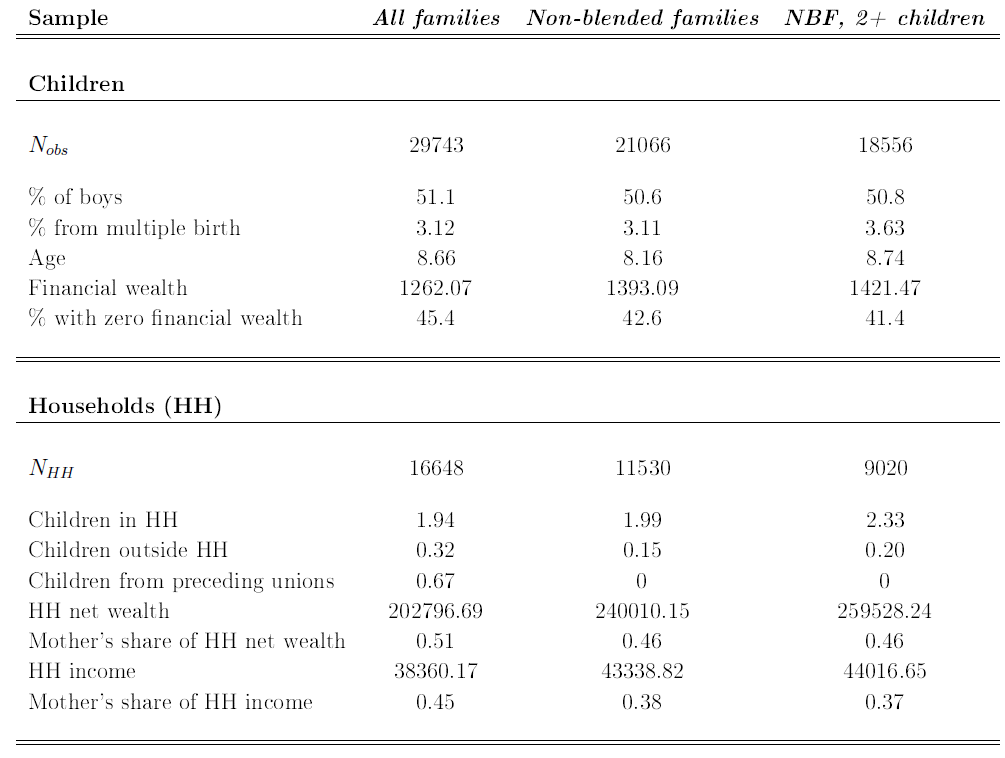
\includegraphics[width = 0.9\textwidth, height = 0.9\textheight, keepaspectratio]{samples.png}
	\end{figure}
\end{frame}

%%%%%%%%%%	Dependent / independent variable

\begin{frame}[label = dep_indep]{Limits \& questions}    
	\begin{itemize}\setlength{\itemsep}{15pt}
		\item Limits when used as dependent / independent variable $\rightarrow$ same as when working with usual wealth but even more severe (skewed, large share of $0$s, measurement errors, etc.)
		\item Real estate assets highly selected: 1.30\% of children, yielding a mean increase of 25\% from 1262 to 1572 euros 
		\item Endogeneity in a lot of social processes / mechanisms (+ composition effects of HH structures)
		\item Which weights?
	\end{itemize}
\end{frame}

%----------------------------------------------------------------------------------------
%              				RESULTS   
%----------------------------------------------------------------------------------------

\section{Stylized facts \& results}

%%%%%%%%%%	Distribution

\begin{frame}[label = distrib]{Children's wealth distribution}    
	\begin{figure}[h]
		\centering
		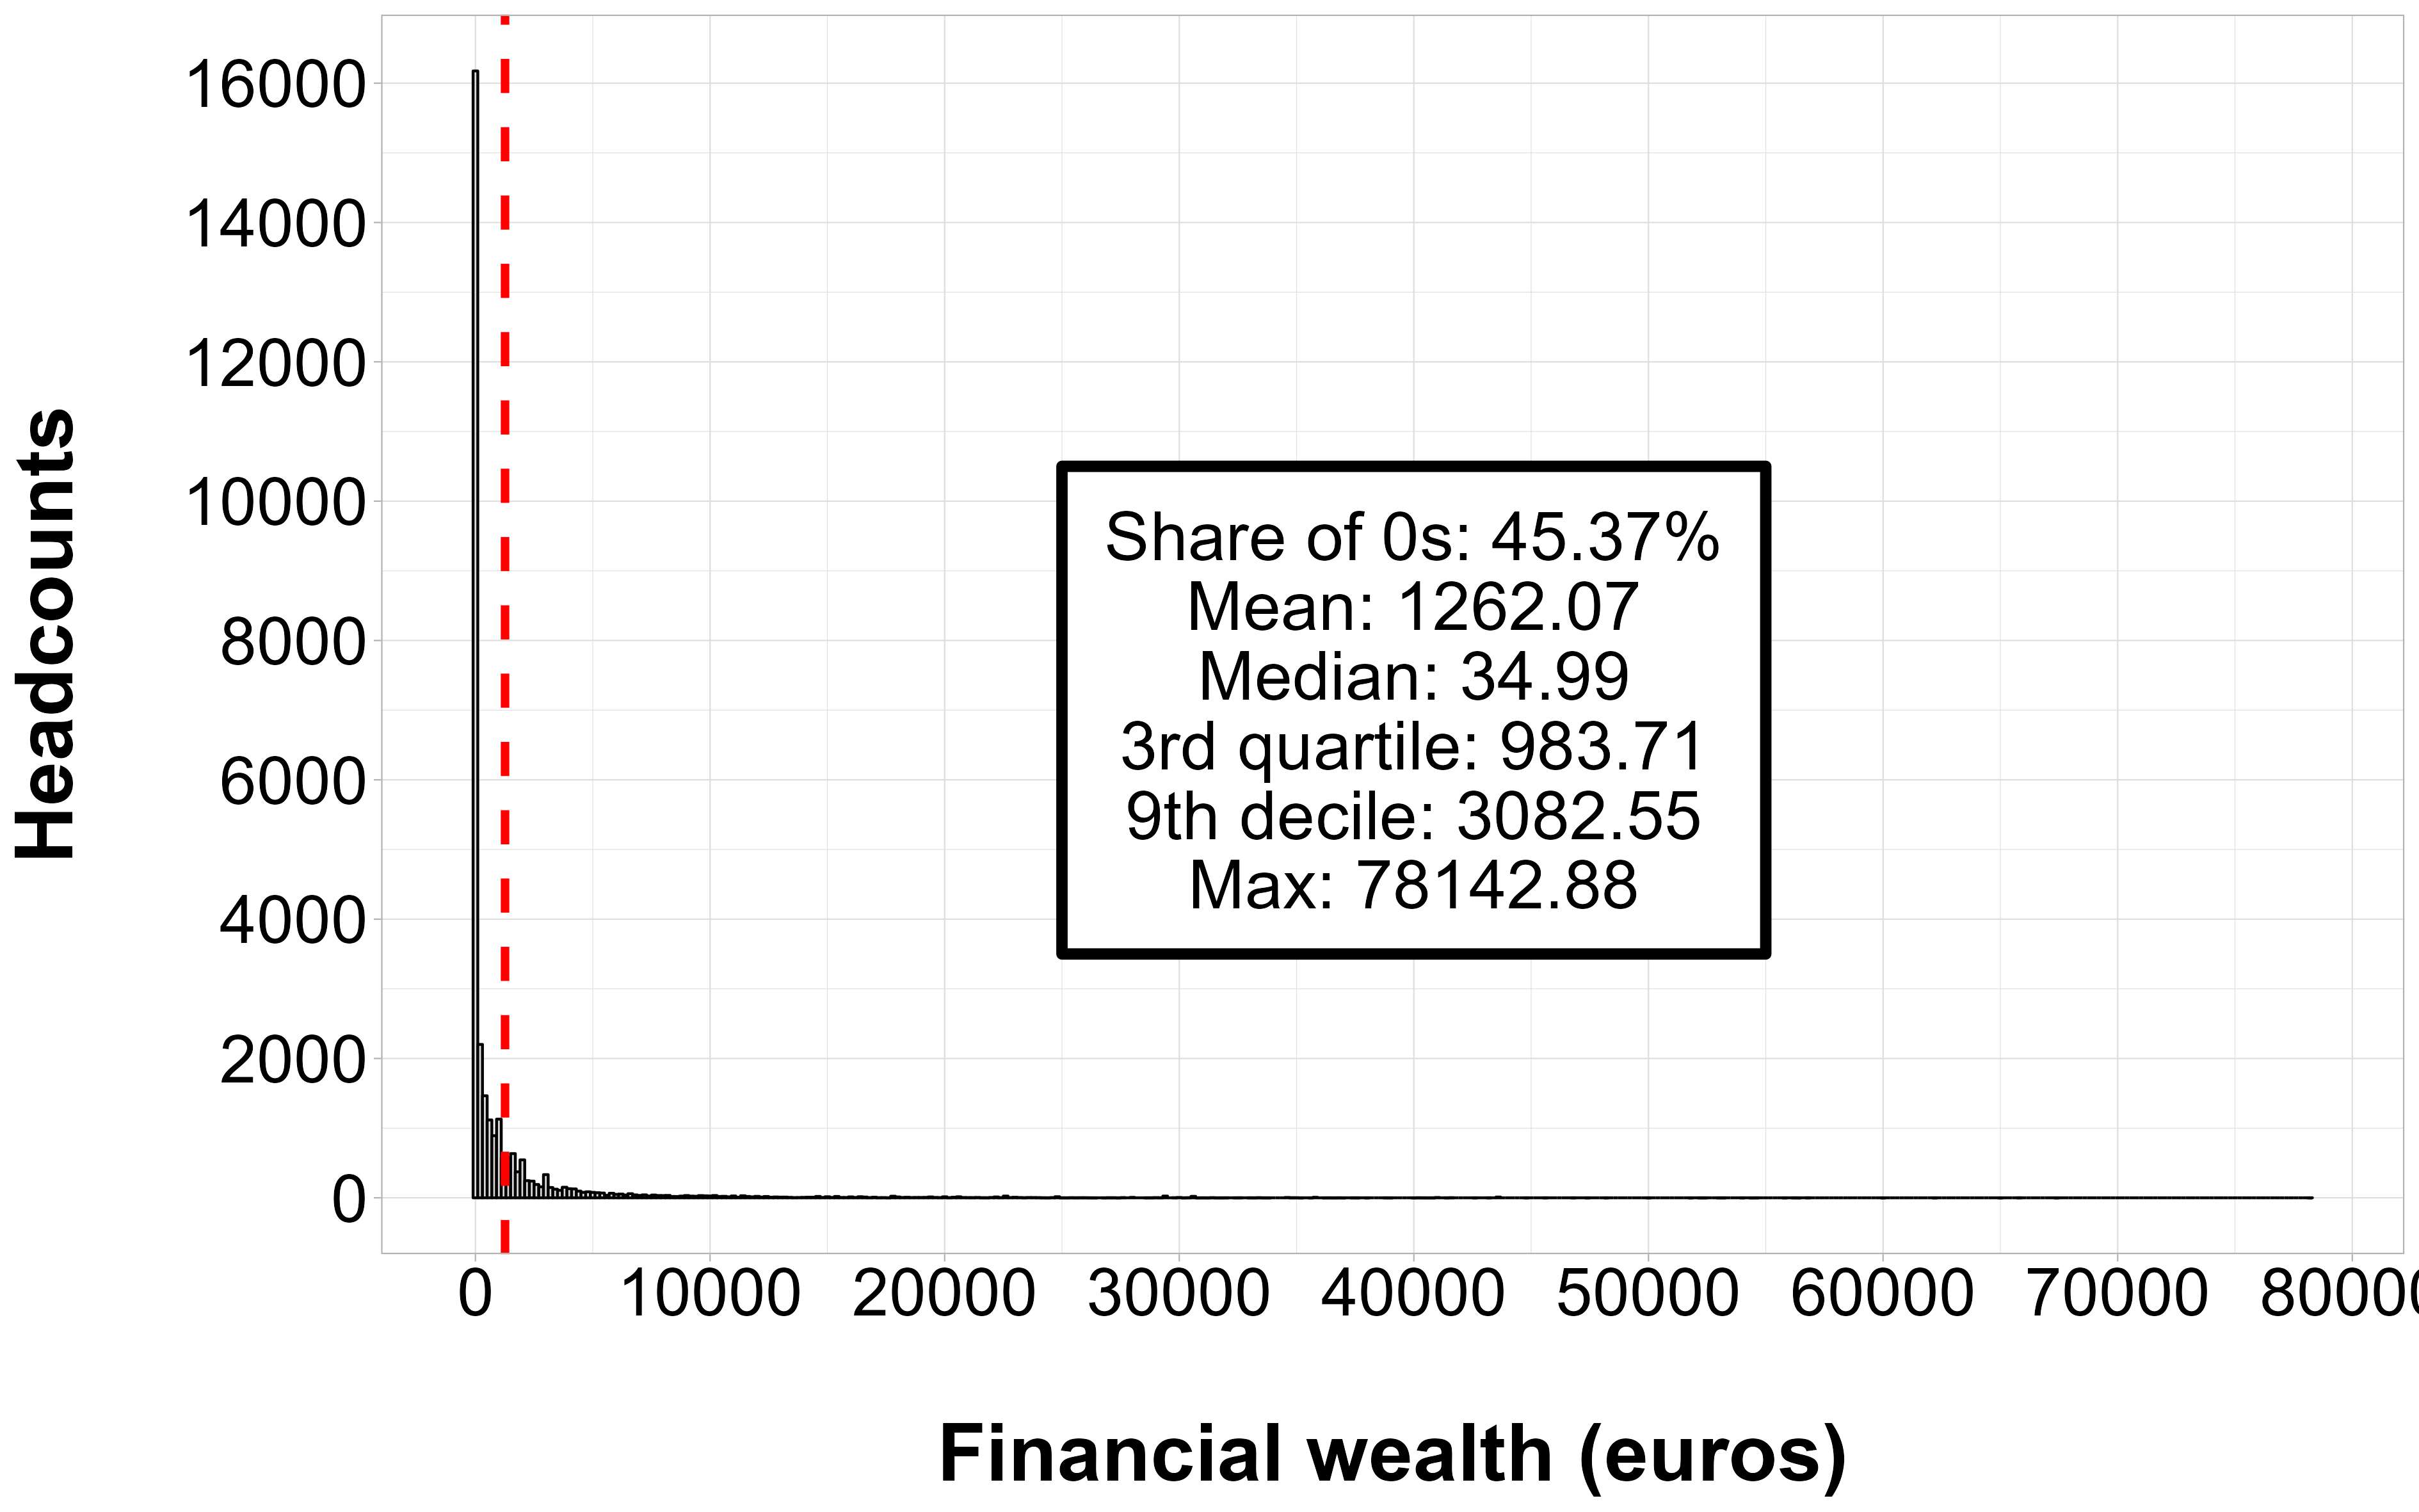
\includegraphics[width = 0.85\textwidth, height = 0.85\textheight, keepaspectratio]{wealthall_distrib_raw.png}
		\caption{\scriptsize{Distribution of financial wealth directly owned by minor children.}}
	\end{figure}
\end{frame}

%%%%%%%%%%	Distribution IHS

\begin{frame}[label = distrib_ihs]{Children's wealth distribution (IHS-transformed)}    
	\begin{figure}[h]
		\centering
		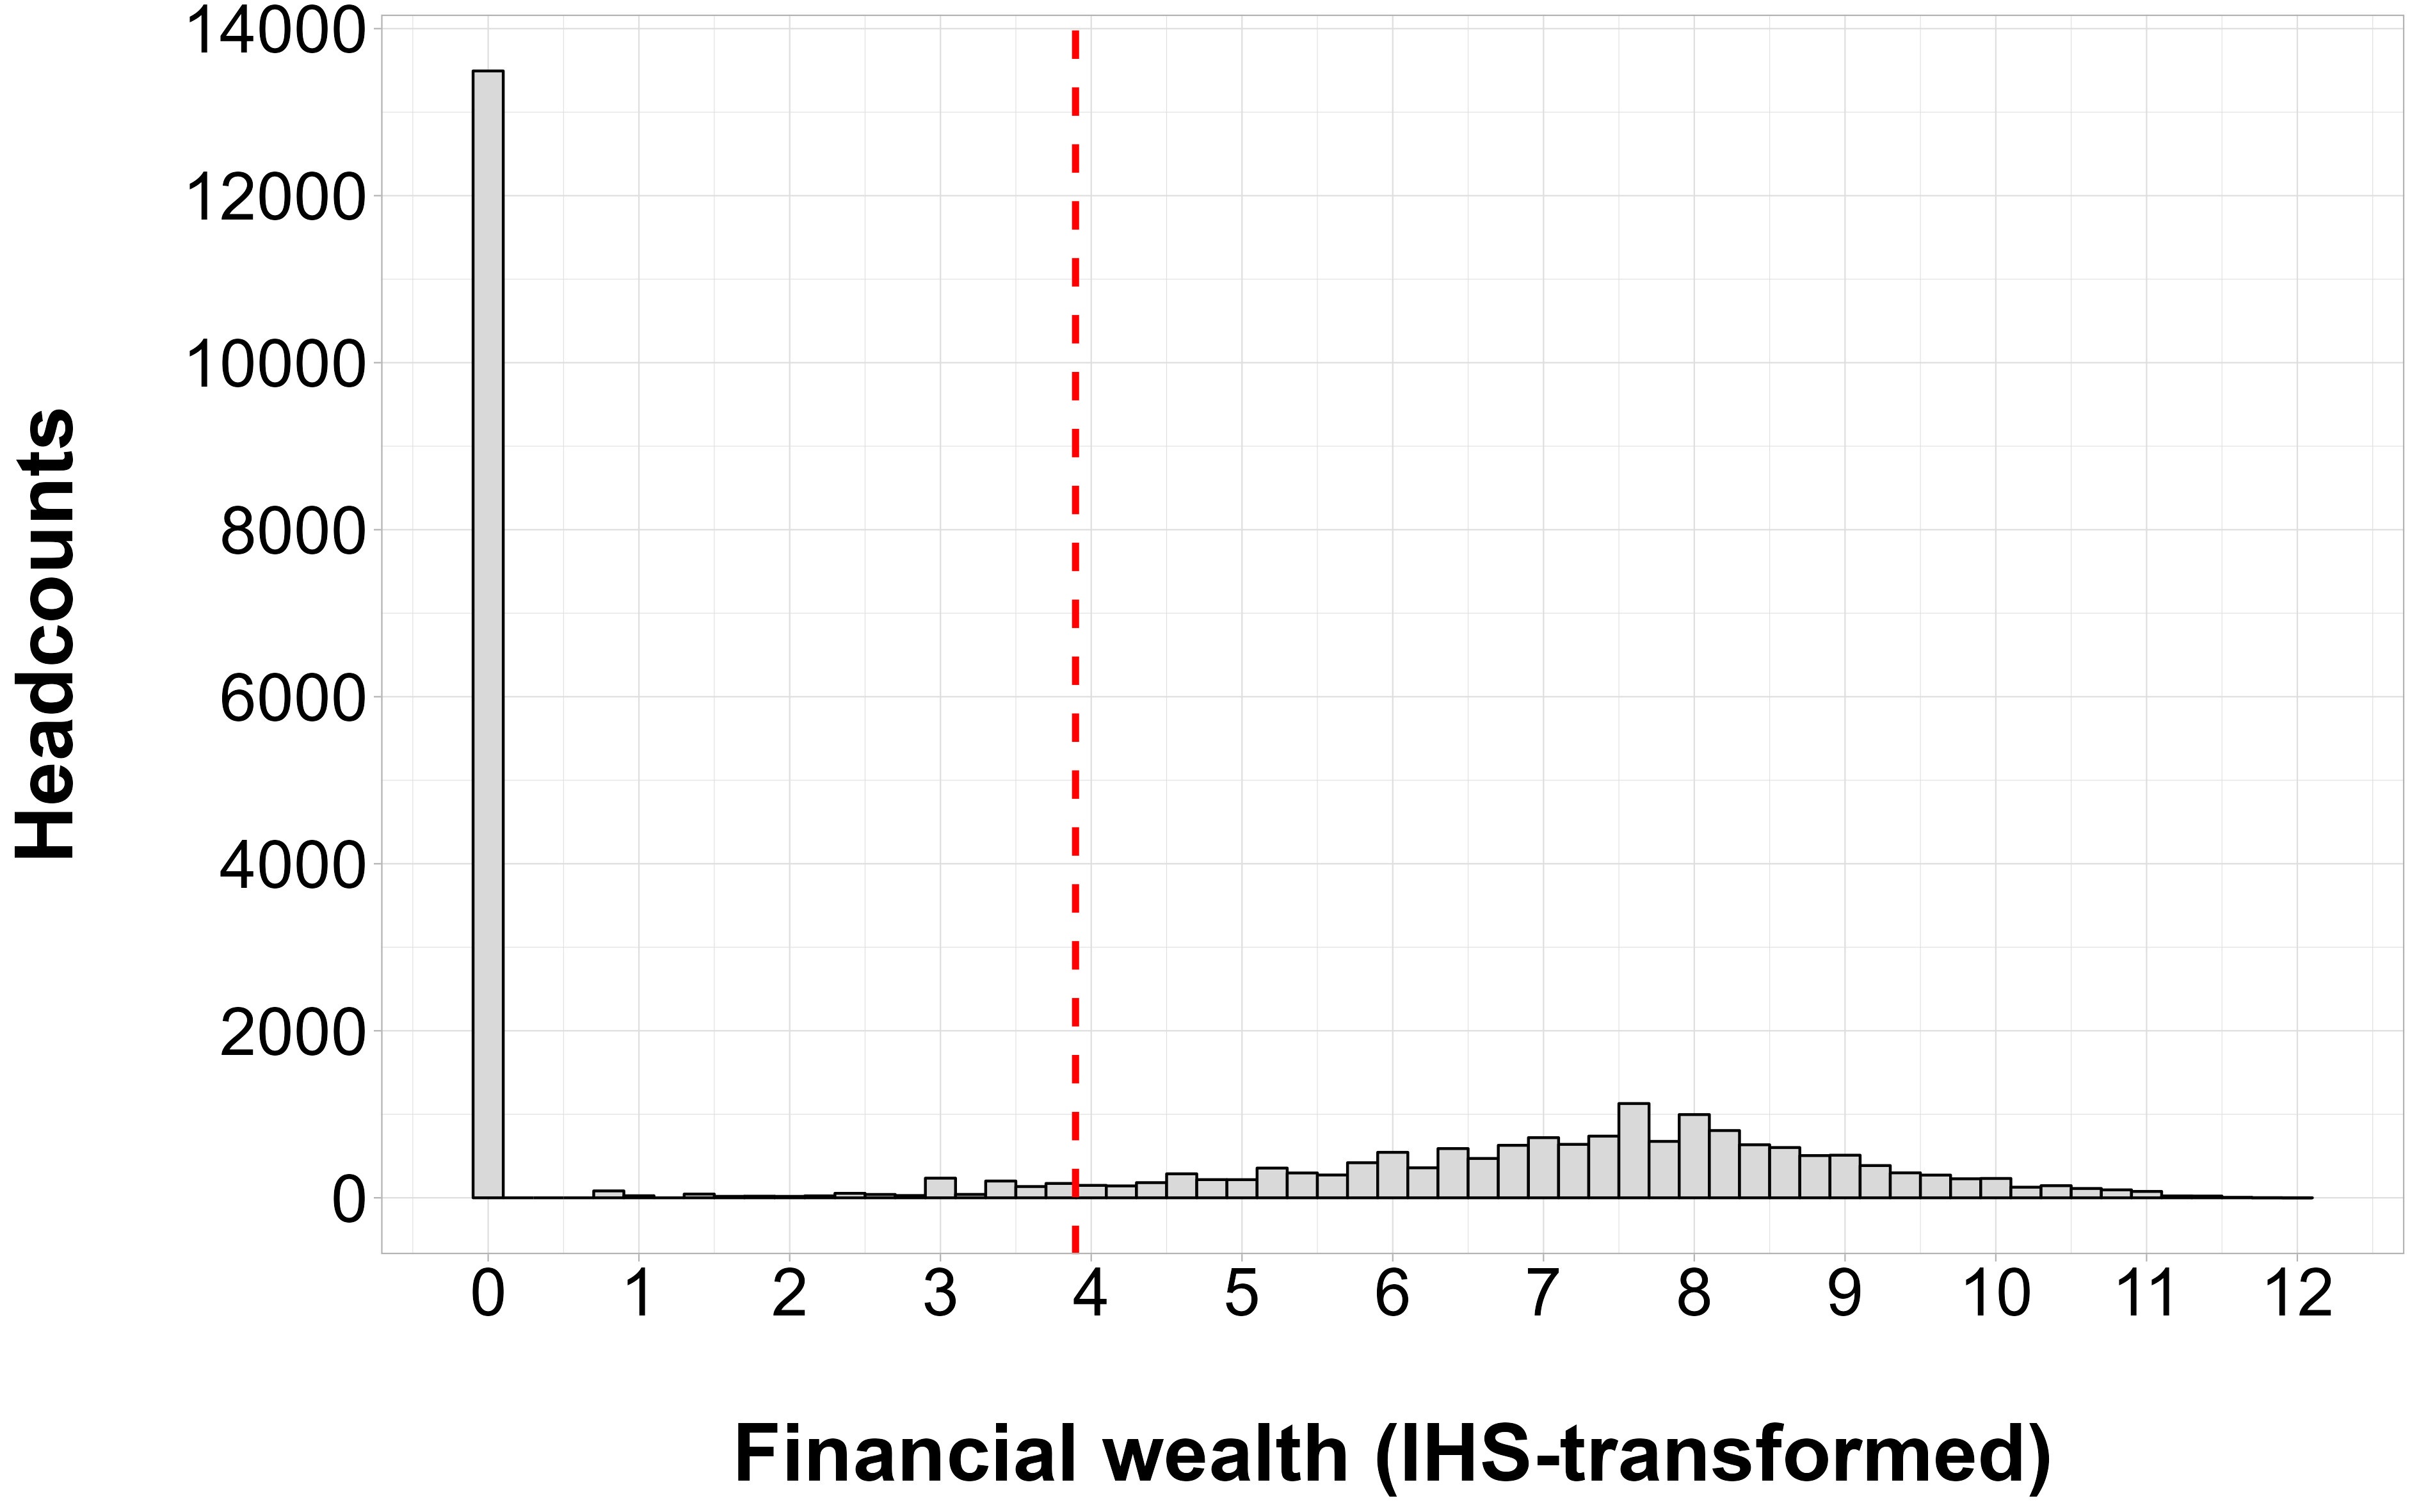
\includegraphics[width = 0.85\textwidth, height = 0.85\textheight, keepaspectratio]{wealthall_distrib_ihs.png}
		\caption{\scriptsize{Distribution of IHS-transformed financial wealth directly owned by minor children.}}
	\end{figure}
\end{frame}

%%%%%%%%%%	Assets

\begin{frame}[label = assets]{Assets}    
	\begin{figure}[h]
		\centering
		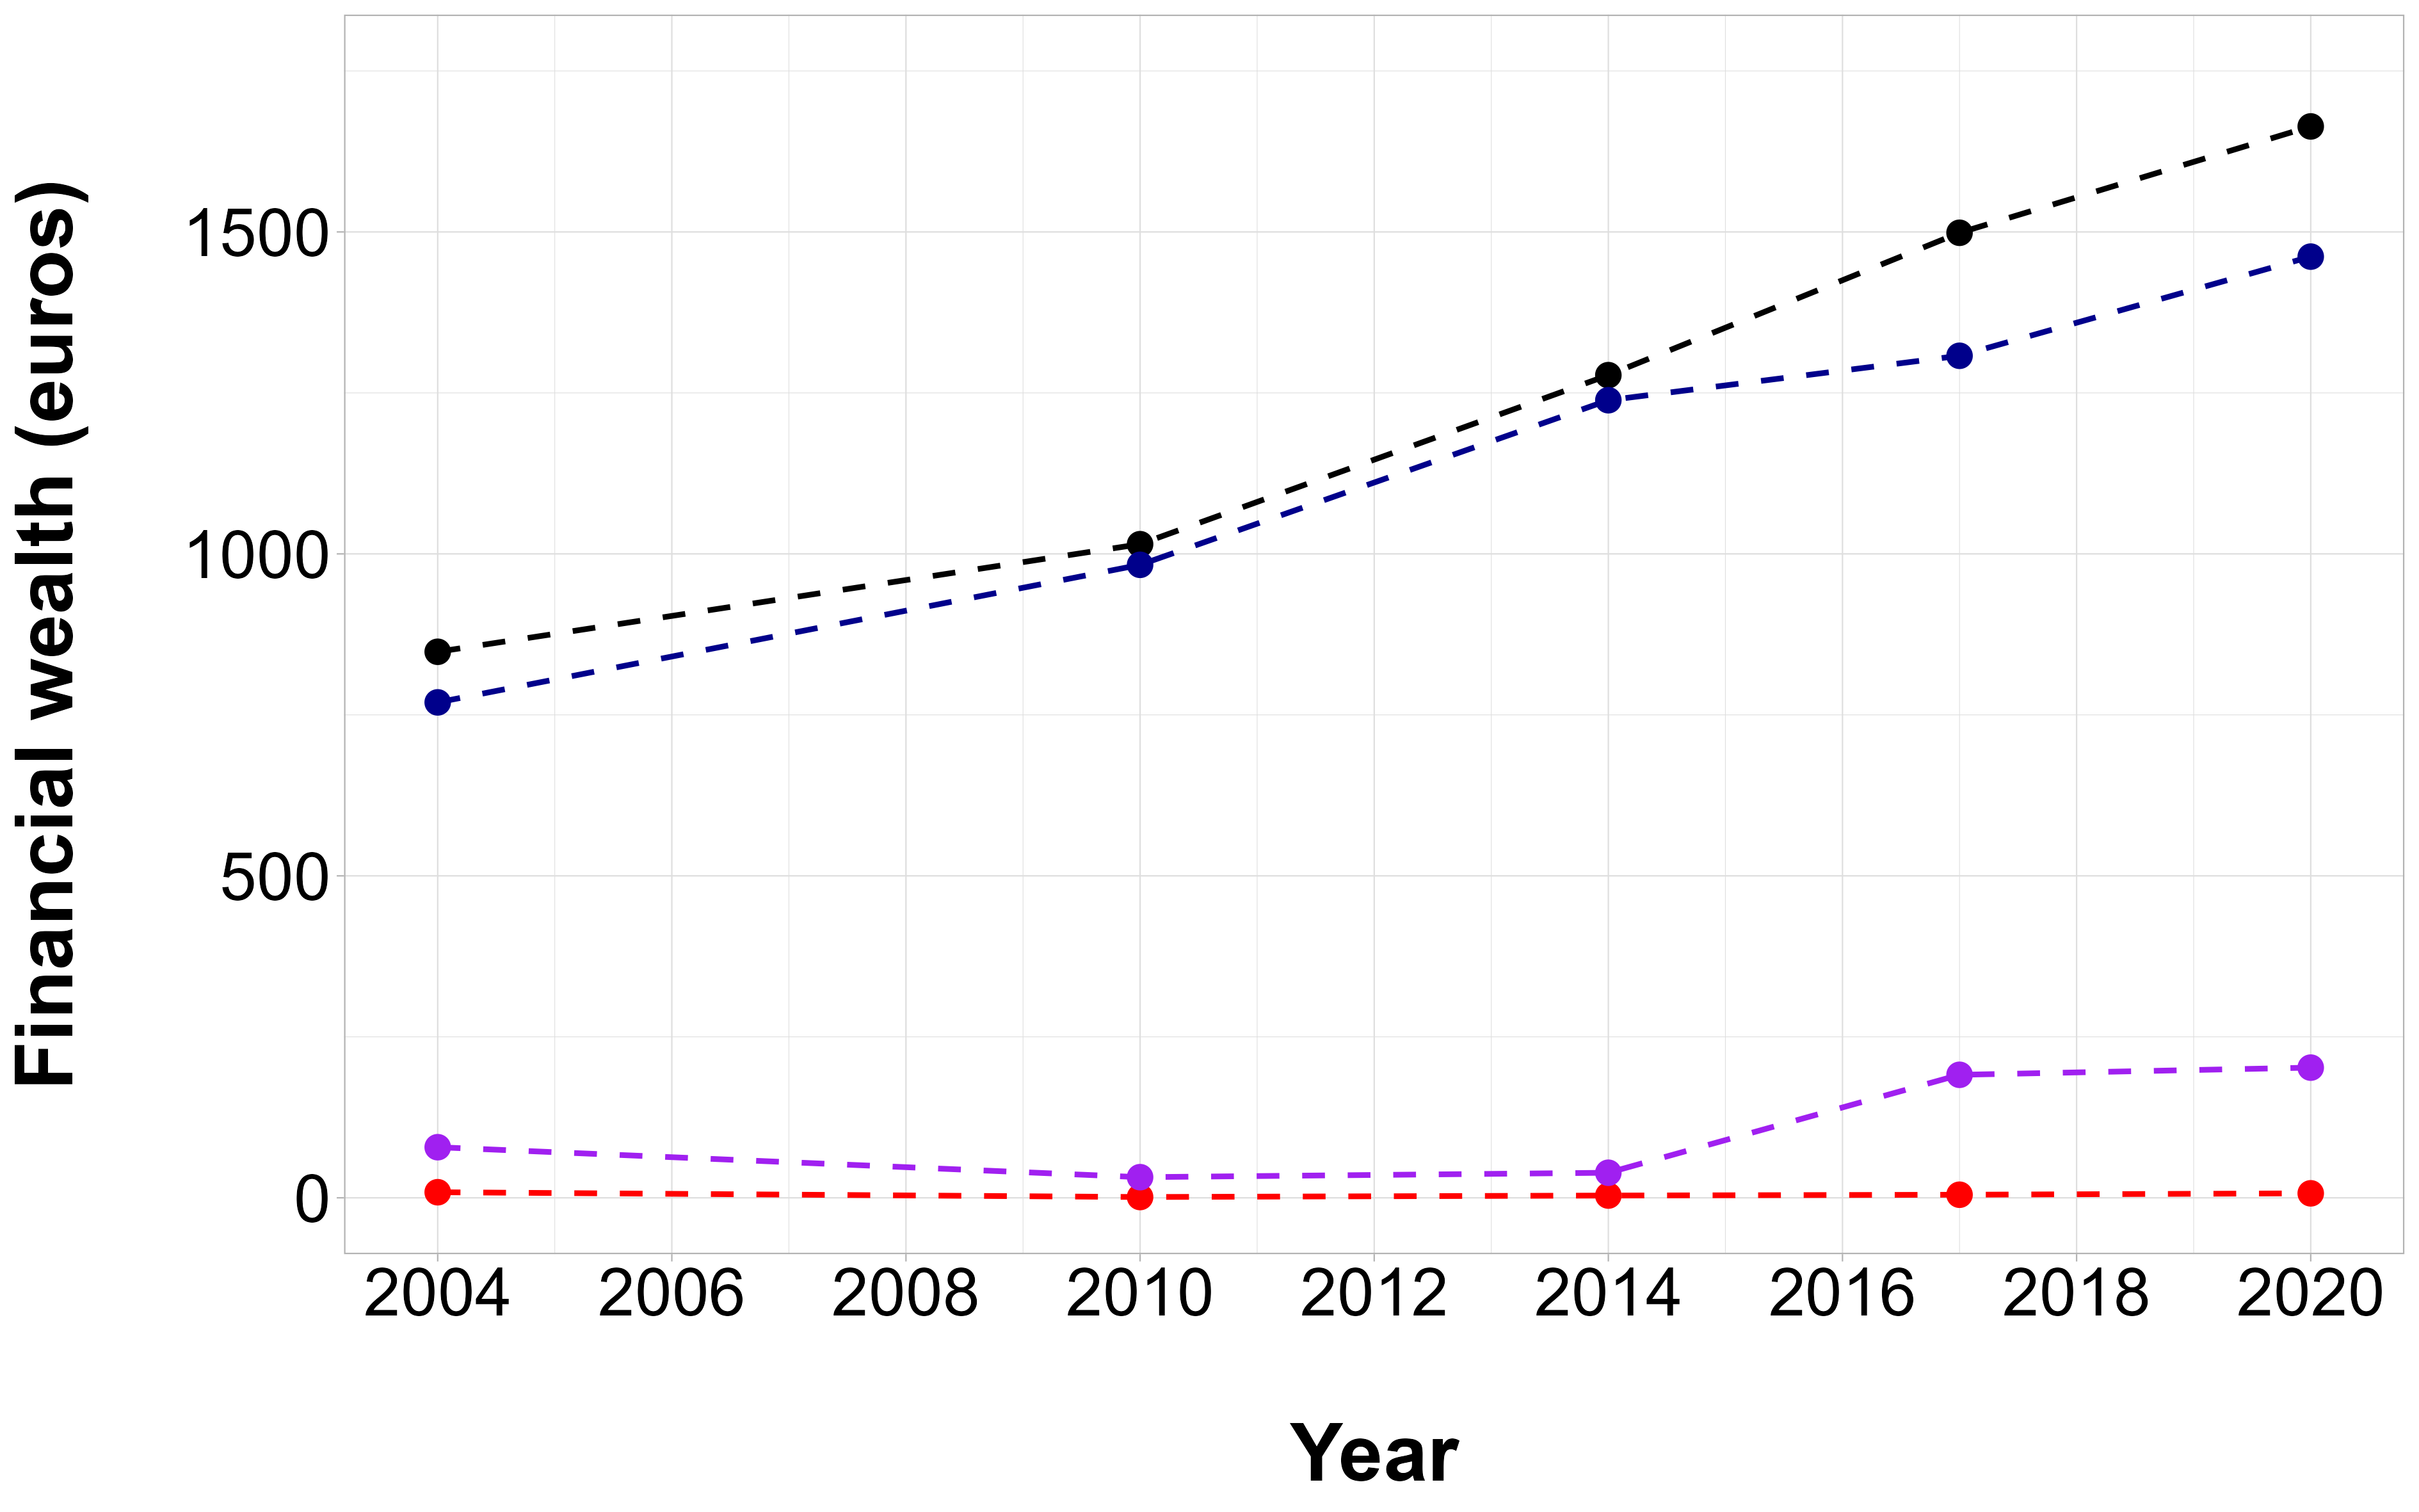
\includegraphics[width = 0.85\textwidth, height = 0.85\textheight, keepaspectratio]{wealthall_time_series_assets.png}
		\caption{\scriptsize{Time-series of mean financial wealth (black), broken down by current accounts (red), savings accounts (blue), non-savings assets (purple).}}
	\end{figure}
\end{frame}


%%%%%%%%%%	CHILDREN CHARACTERISTICS

%%%%%%%%%%	Sibship size & age

\begin{frame}[label = sibhip]{Fewer siblings, more wealth?}       
	\begin{figure}[h]
		\centering
		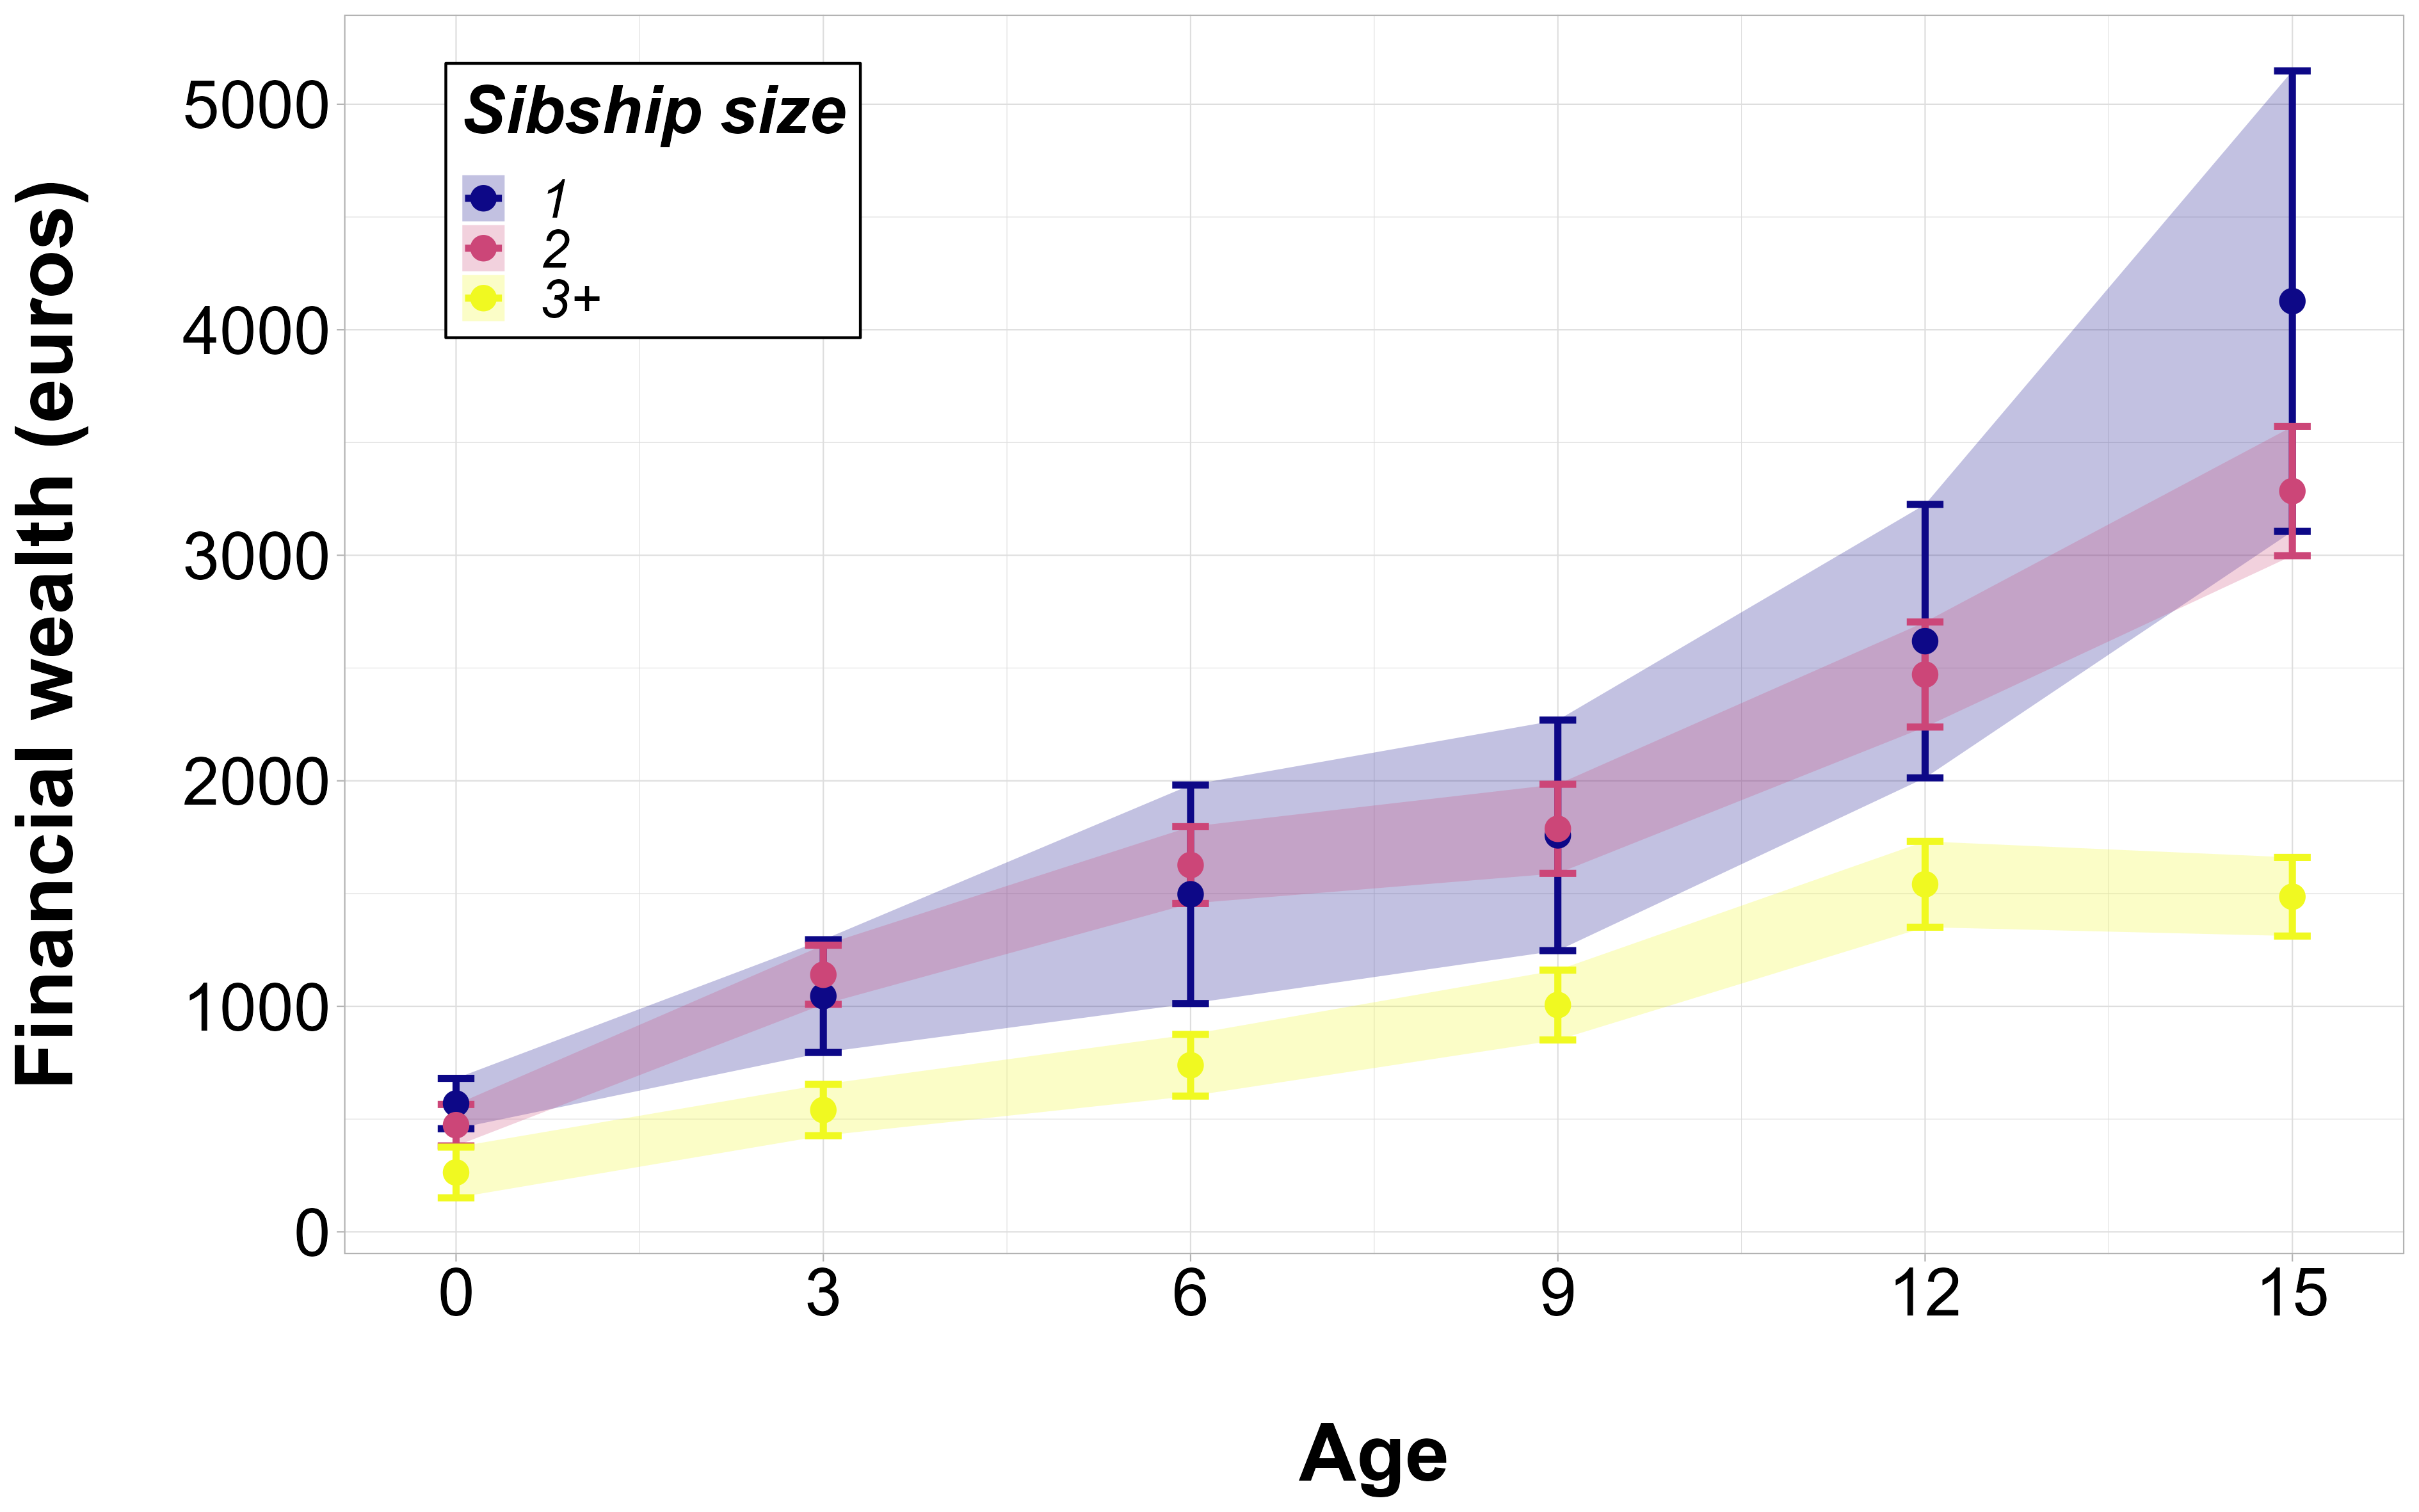
\includegraphics[width = 0.85\textwidth, height = 0.85\textheight, keepaspectratio]{wealth_age3_sibsize3_all.png}
		\vspace{-0.3cm}
		\caption*{\tiny{Colored areas represent 95\% confidence intervals.}}
		\vspace{-0.5cm}
		\caption{\scriptsize{Mean financial wealth by age according to sibship size.
		\\
		Observations here are restricted to the subsample of non-blended families.}}
	\end{figure}
\end{frame}

%%%%%%%%%%	Gender & sibship size & age

\begin{frame}[label = gender_sibhip]{No visible gender differences}    
	\begin{figure}[h]
		\centering
		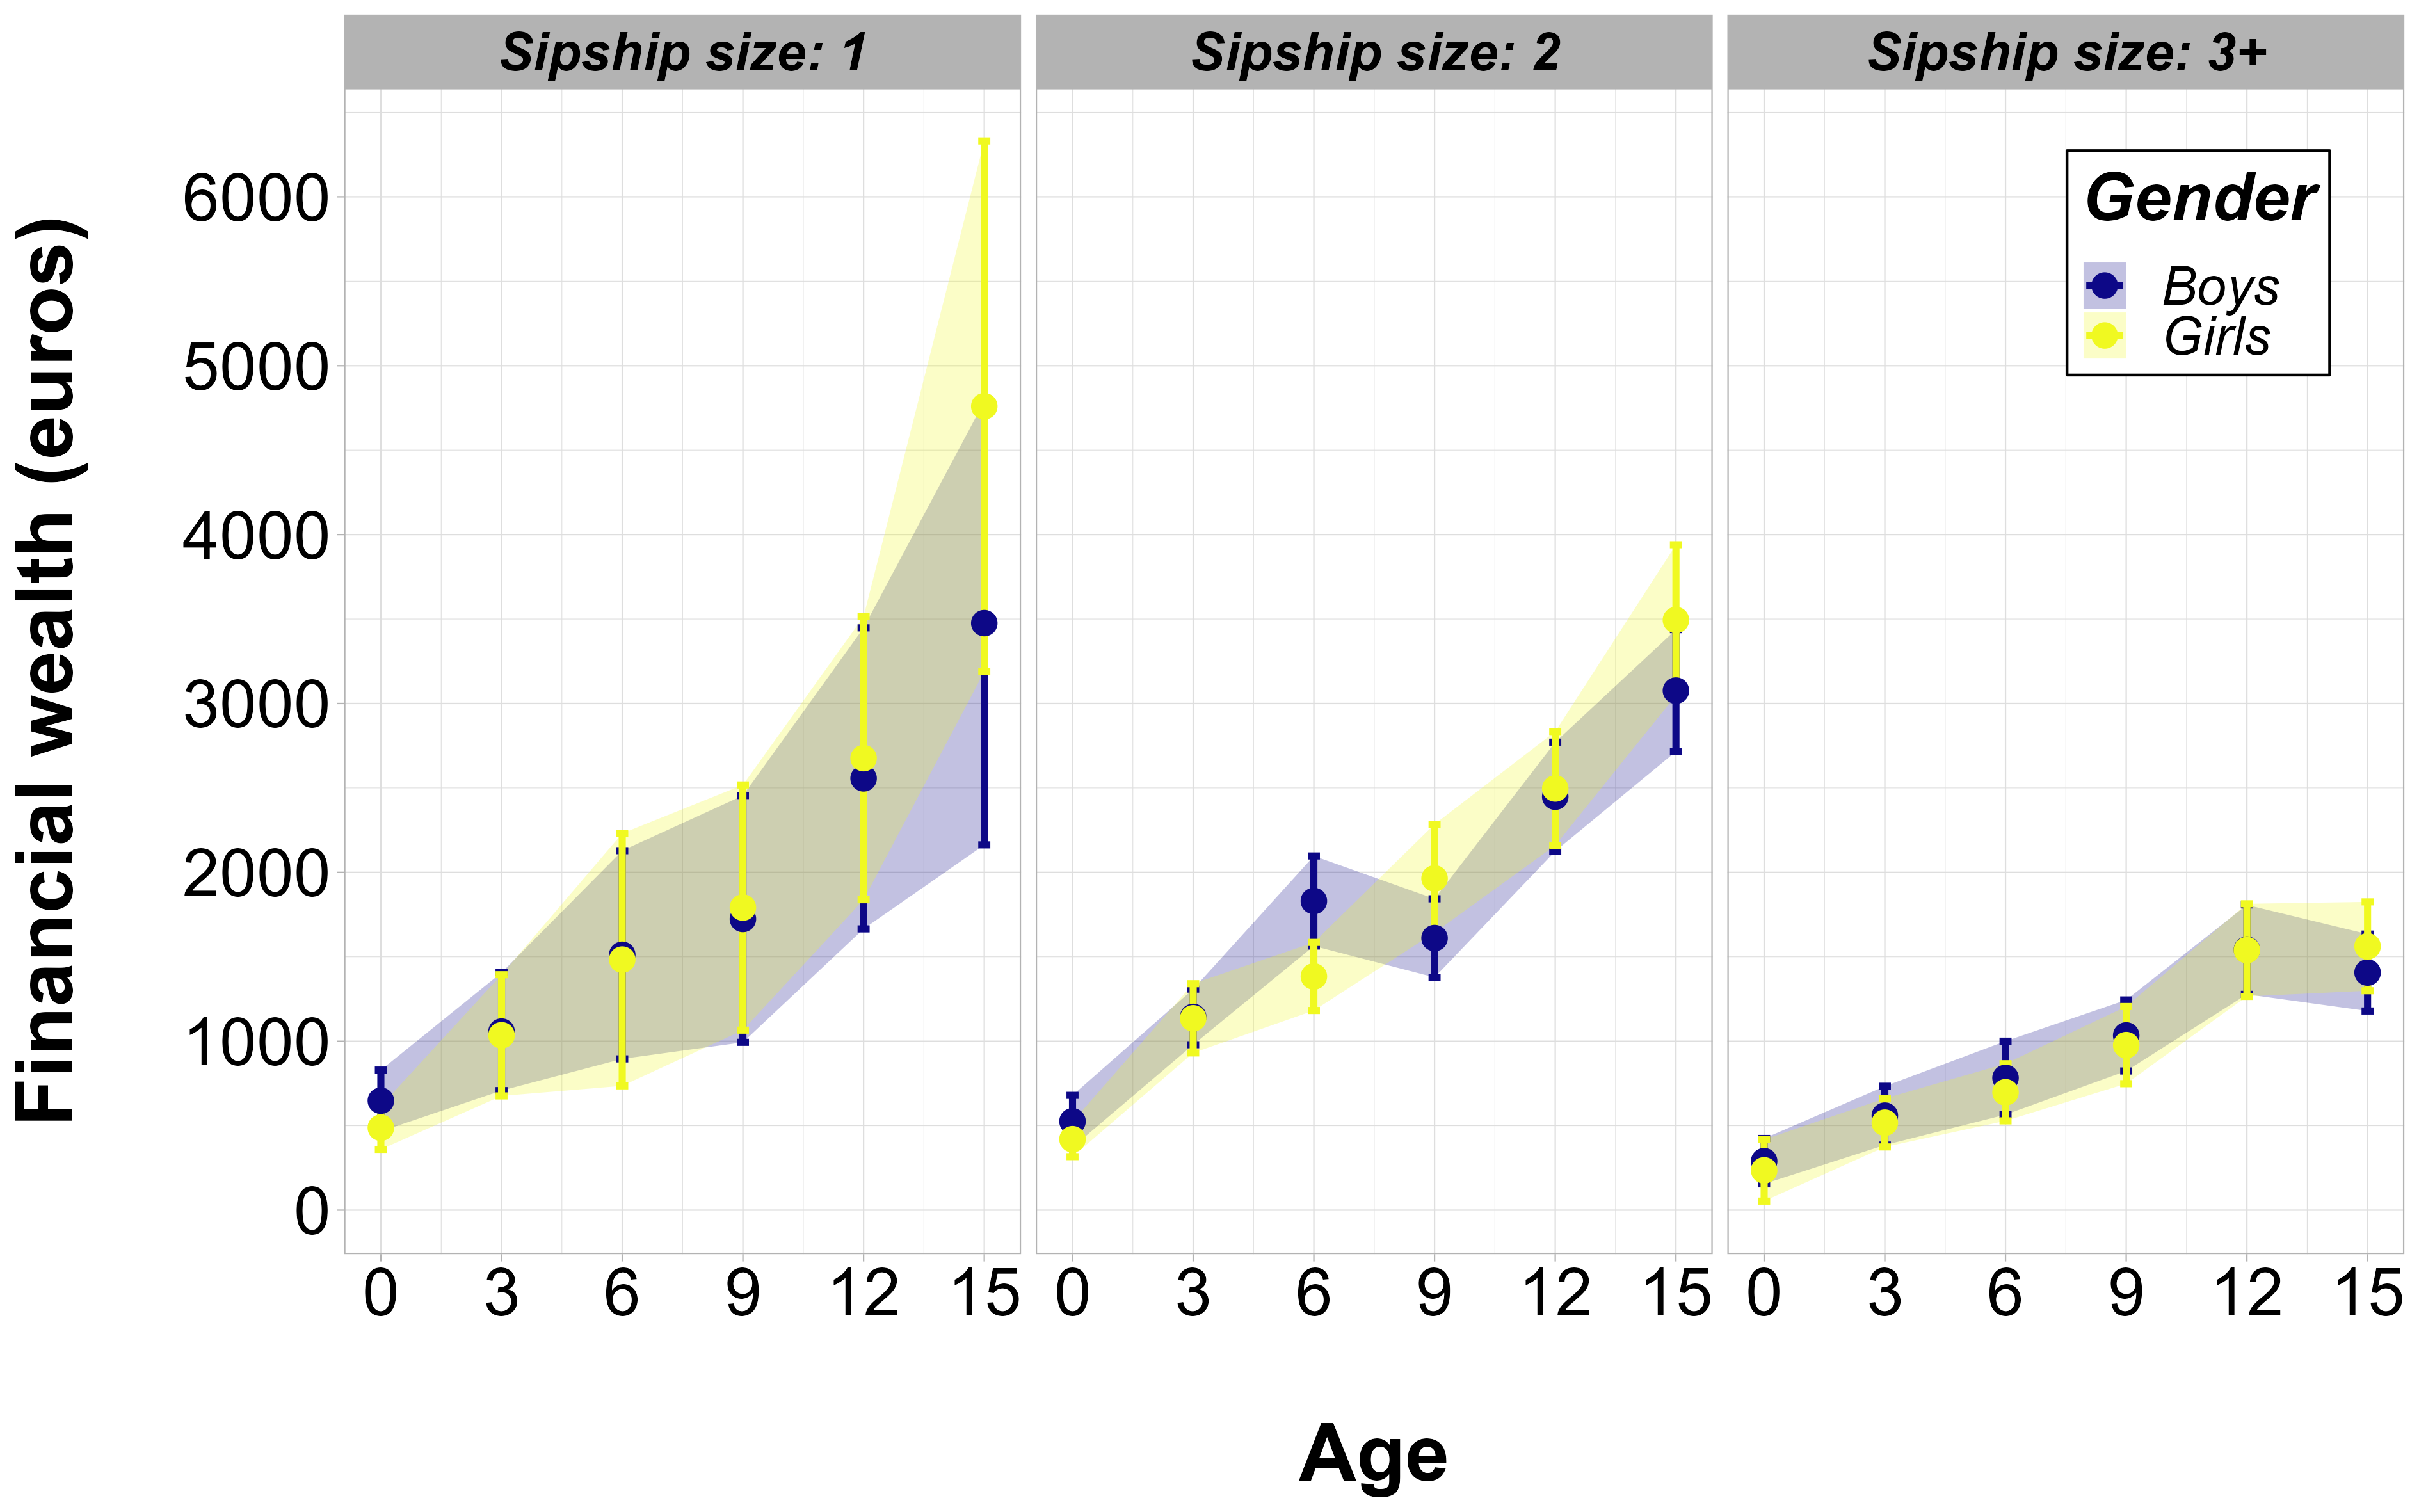
\includegraphics[width = 0.85\textwidth, height = 0.85\textheight, keepaspectratio]{wealth_age3_sexe_sibsize3_within.png}
		\vspace{-0.3cm}
		\caption*{\tiny{Colored areas represent 95\% confidence intervals.}}
		\vspace{-0.5cm}
		\caption{\scriptsize{Mean financial wealth by age according to sibship size, broken down by gender.
		\\
		Observations here are restricted to the subsample of non-blended families.}}
	\end{figure}
\end{frame}

%%%%%%%%%%	Rank & sibship size & age

\begin{frame}[label = rank_sibhip]{No visible rank differences}    
	\begin{figure}[h]
		\centering
		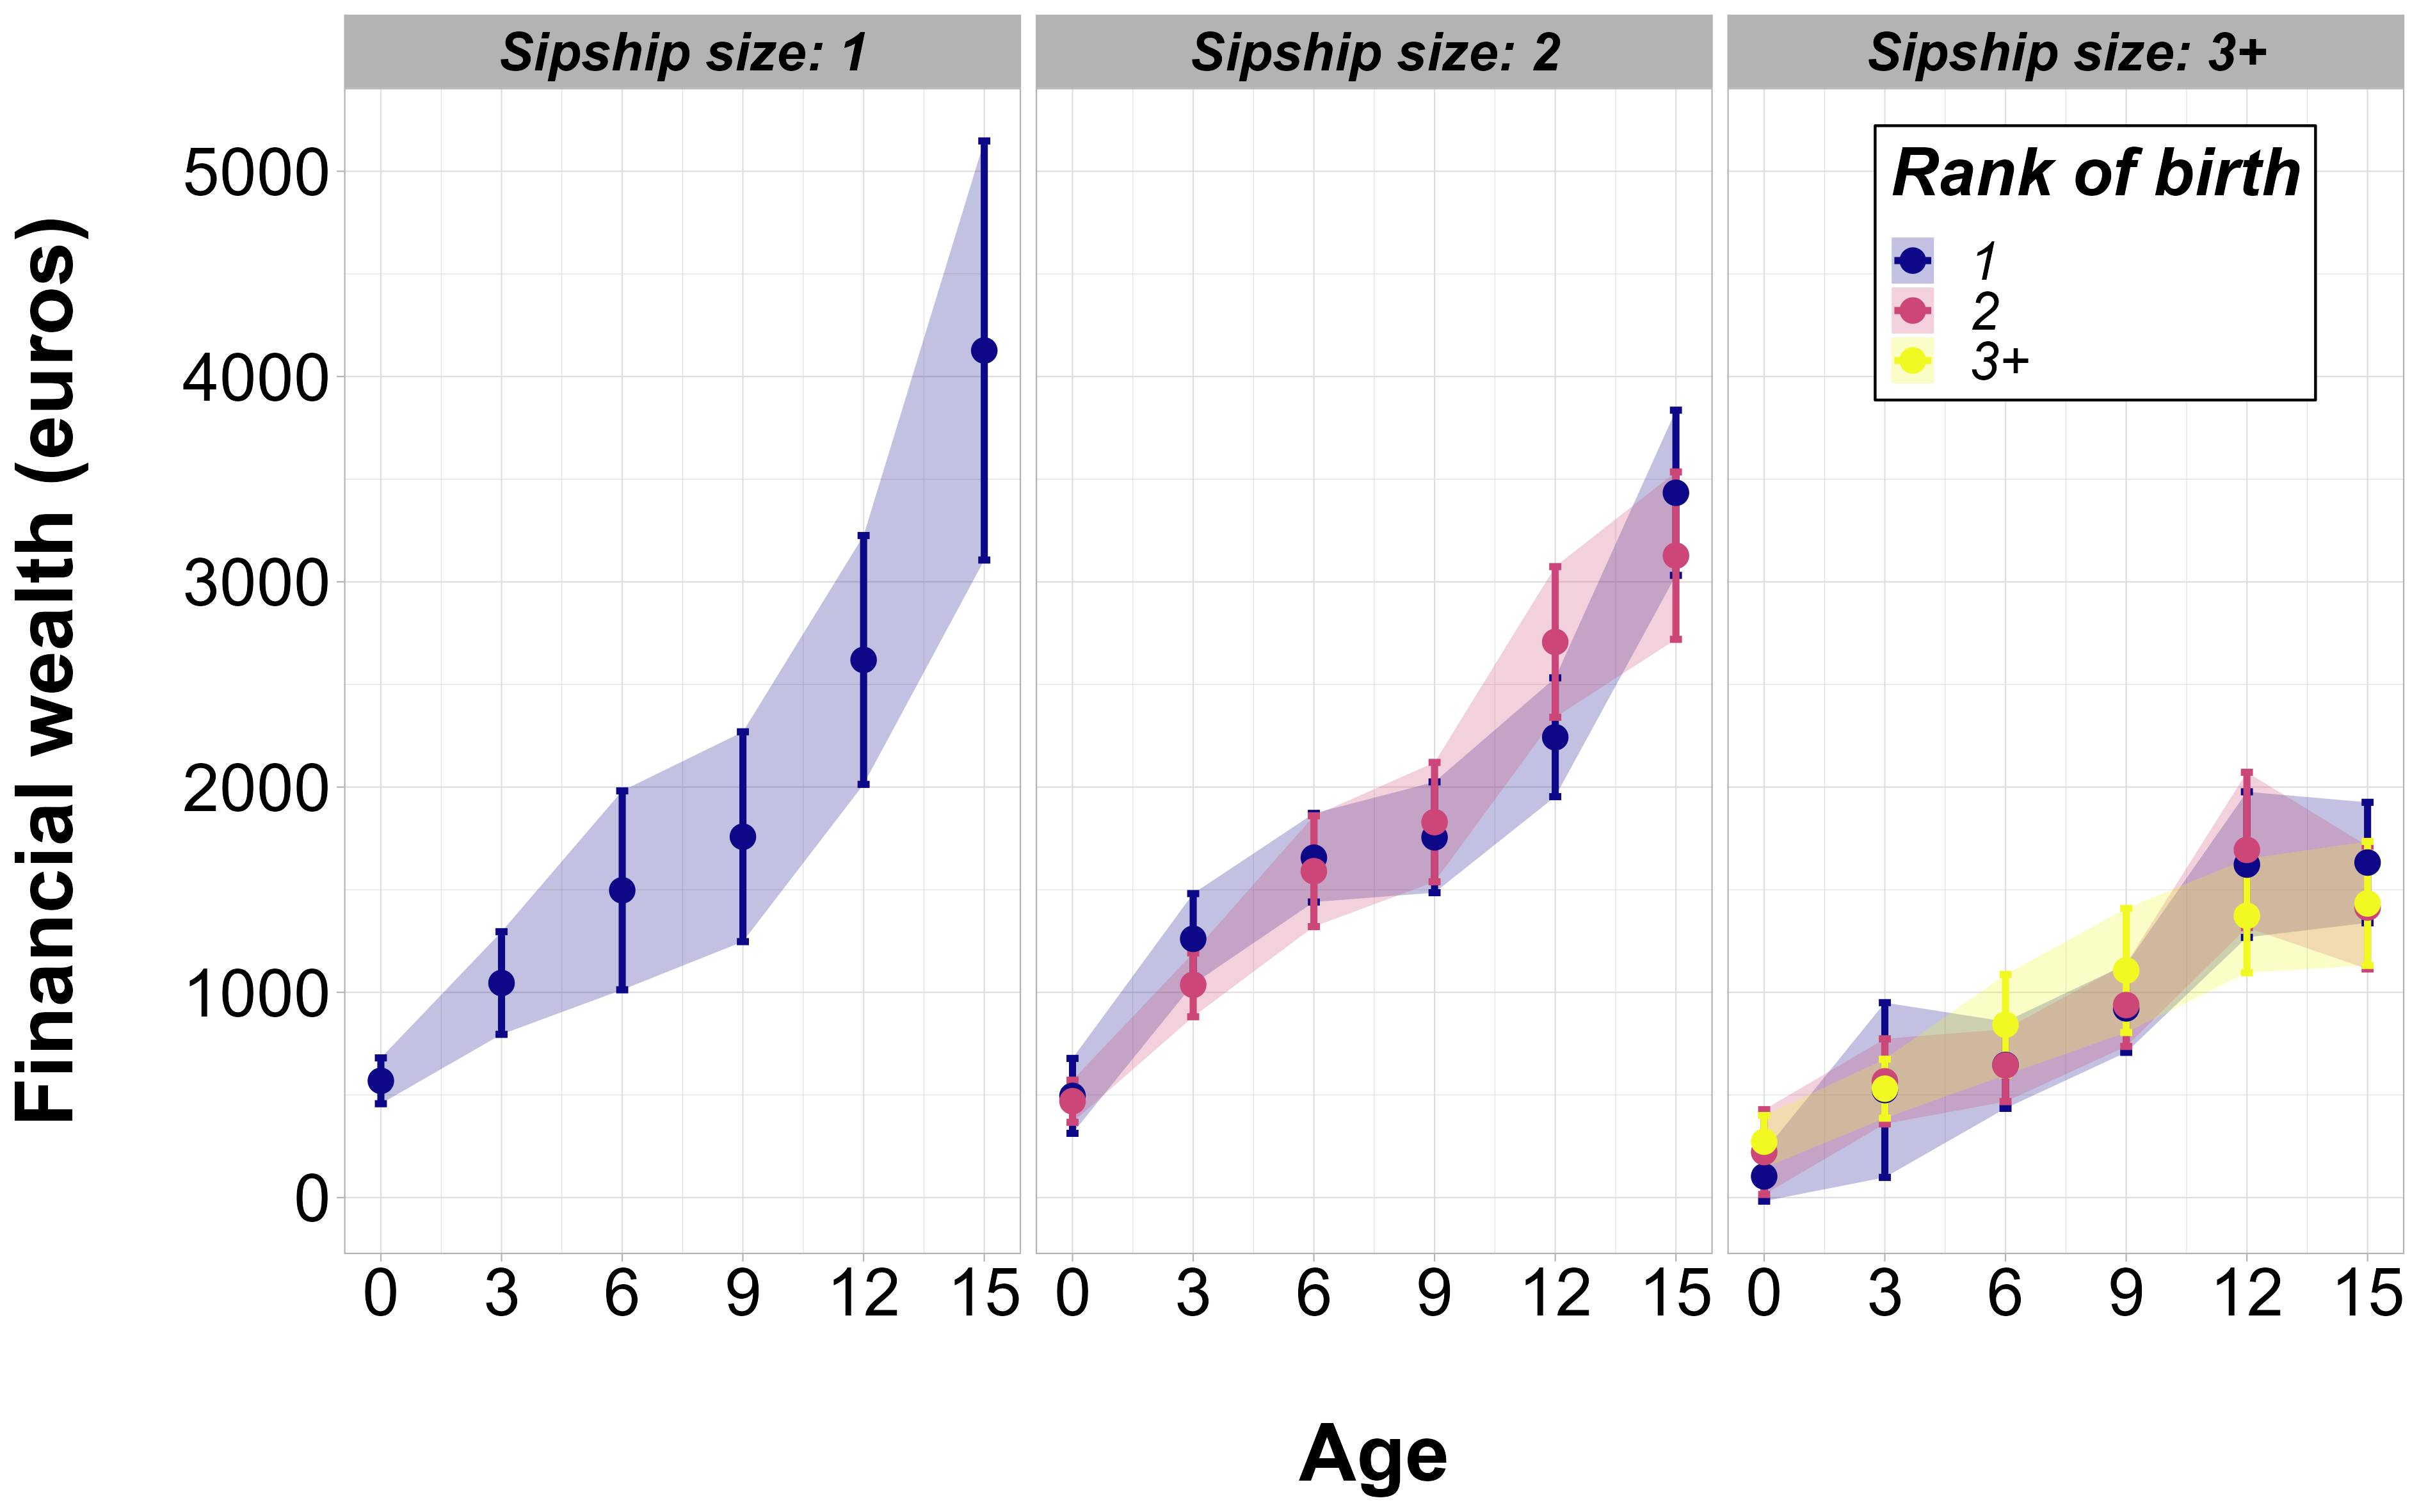
\includegraphics[width = 0.85\textwidth, height = 0.85\textheight, keepaspectratio]{wealth_age3_rank3_sibsize3_within.png}
		\vspace{-0.3cm}
		\caption*{\tiny{Colored areas represent 95\% confidence intervals.}}
		\vspace{-0.5cm}
		\caption{\scriptsize{Mean financial wealth by age according to sibship size, broken down by rank of birth.
		\\
		Observations here are restricted to the subsample of non-blended families.}}
	\end{figure}
\end{frame}

%%%%%%%%%%	Intergenerational mobilty

\begin{frame}[label = boserup]{\citet{boserup_born_2018}}    
\begin{figure}[ht]
        \begin{minipage}[b]{0.45\linewidth}
            \centering
            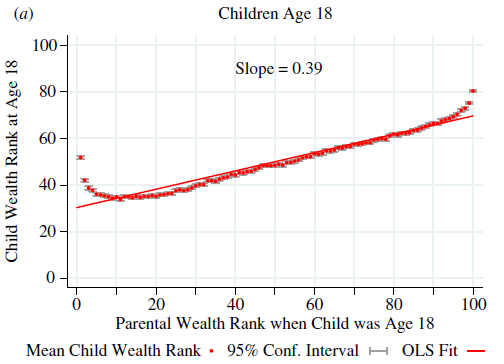
\includegraphics[width=\textwidth]{Boserup_a.png}
        \end{minipage}
        \hspace{0.2cm}
        \begin{minipage}[b]{0.45\linewidth}
            \centering
            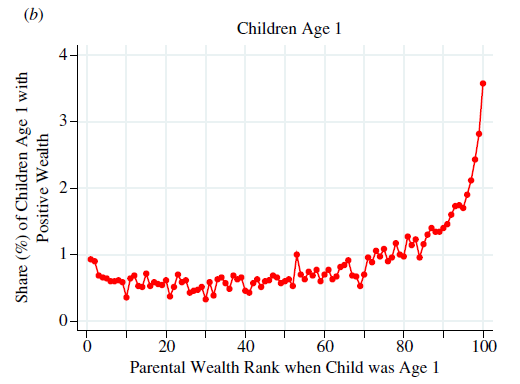
\includegraphics[width=\textwidth]{Boserup_b.png}
        \end{minipage}
		\caption{\scriptsize{Relationship of Parental and Childhood Wealth.}}
    \end{figure}
\end{frame}


%----------------------------------------------------------------------------------------
%              			REFERENCES   
%----------------------------------------------------------------------------------------

\begin{frame}[allowframebreaks]
\frametitle{References}
\printbibliography
\end{frame}

%%%%%%%%%%


\end{document}














